\section{Constant Phase Shifter}
\label{sec:constant-phase-shifter}
%
A constant phase shifter, also known as fractional Hilbert transformer~\cite{lohmann1996},
refers to a filter that applies a (frequency independent) constant shift $\varphi$
to the spectrum of an input signal.
This section introduces the time and frequency representations
of discrete-time constant phase shifters for aperiodic and periodic signals.
Practical implementations for the respective cases are also discussed.
Since the primary interest of the present study is the audibility of a phase shift,
the main consideration is the accuracy of the constant phase shifter
in terms of its magnitude and phase response.
Computational cost and algorithm optimization are less of a concern.

\subsection[Aperiodic Signals]{Aperiodic Signals}
\label{sec:aperiodic-signals}
%
The transfer function of a constant phase shifter
in the discrete time Fourier transform (DTFT) domain reads
\begin{align}
H(e^{i\Omega}) &=
\begin{cases}
e^{+i\varphi}, & 0 < \Omega < \pi\\
e^{-i\varphi}, & -\pi < \Omega < 0\\
\cos\varphi, & \Omega = 0, \pi
\end{cases}
\label{eq:def-dtft}
\end{align}
where $\Omega = \frac{2\pi f}{\fs}$ denotes the normalized angular frequency
for the sampling rate $\fs$.
By exploiting Euler's formula, \eqref{eq:def-dtft} can be decomposed into
\begin{align}
H(e^{i\Omega})
= \cos\varphi
- \sin\varphi\cdot\Hh(e^{i\Omega}),
\label{eq:decomp-dtft}
\end{align}
with
$\Hh(e^{i\Omega})\coloneqq-i\cdot\sgn{\Omega}$ denoting
the transfer function of the Hilbert transformer~\cite{hahn1996hilbert}.
Notice that the Hilbert transformer can be regarded
as a constant phase shifter of $\varphi=-\tfrac{\pi}{2}$.
Since $\Hh(e^{i\Omega})$ is free of DC bias~\cite[Sec.~4.2]{hahn1996hilbert},
the magnitude response of a constant phase shifter
is unity at all frequencies but $\Omega=0, \pi$,
as given in \eqref{eq:def-dtft}.
%
\begin{figure*}[t]
\centering
\includegraphics[width=\linewidth]{graphics/discrete-irs-phi-45.pdf}
\caption{Left: Impulse response of a constant phase shifter ($\varphi=-45\degree$)
described in \eqref{eq:discrete-ir}.
Center \& Right: Impulse responses of periodic constant phase shifter ($\varphi=-45\degree$)
for even and odd period $M$, described in \eqref{eq:hperi-even} and \eqref{eq:hperi-odd}, respectively.
The coefficients $h[0] = \hperi[0] = \cos\varphi$ are indicated by \stem{colzero}.
The coefficients for $n\neq 0$ indicated by \stem{colnonzero} show
the Hilbert transform part of the impulse response.}
\label{fig:discrete-ir}
\end{figure*}
%
\begin{figure*}[]
\centering
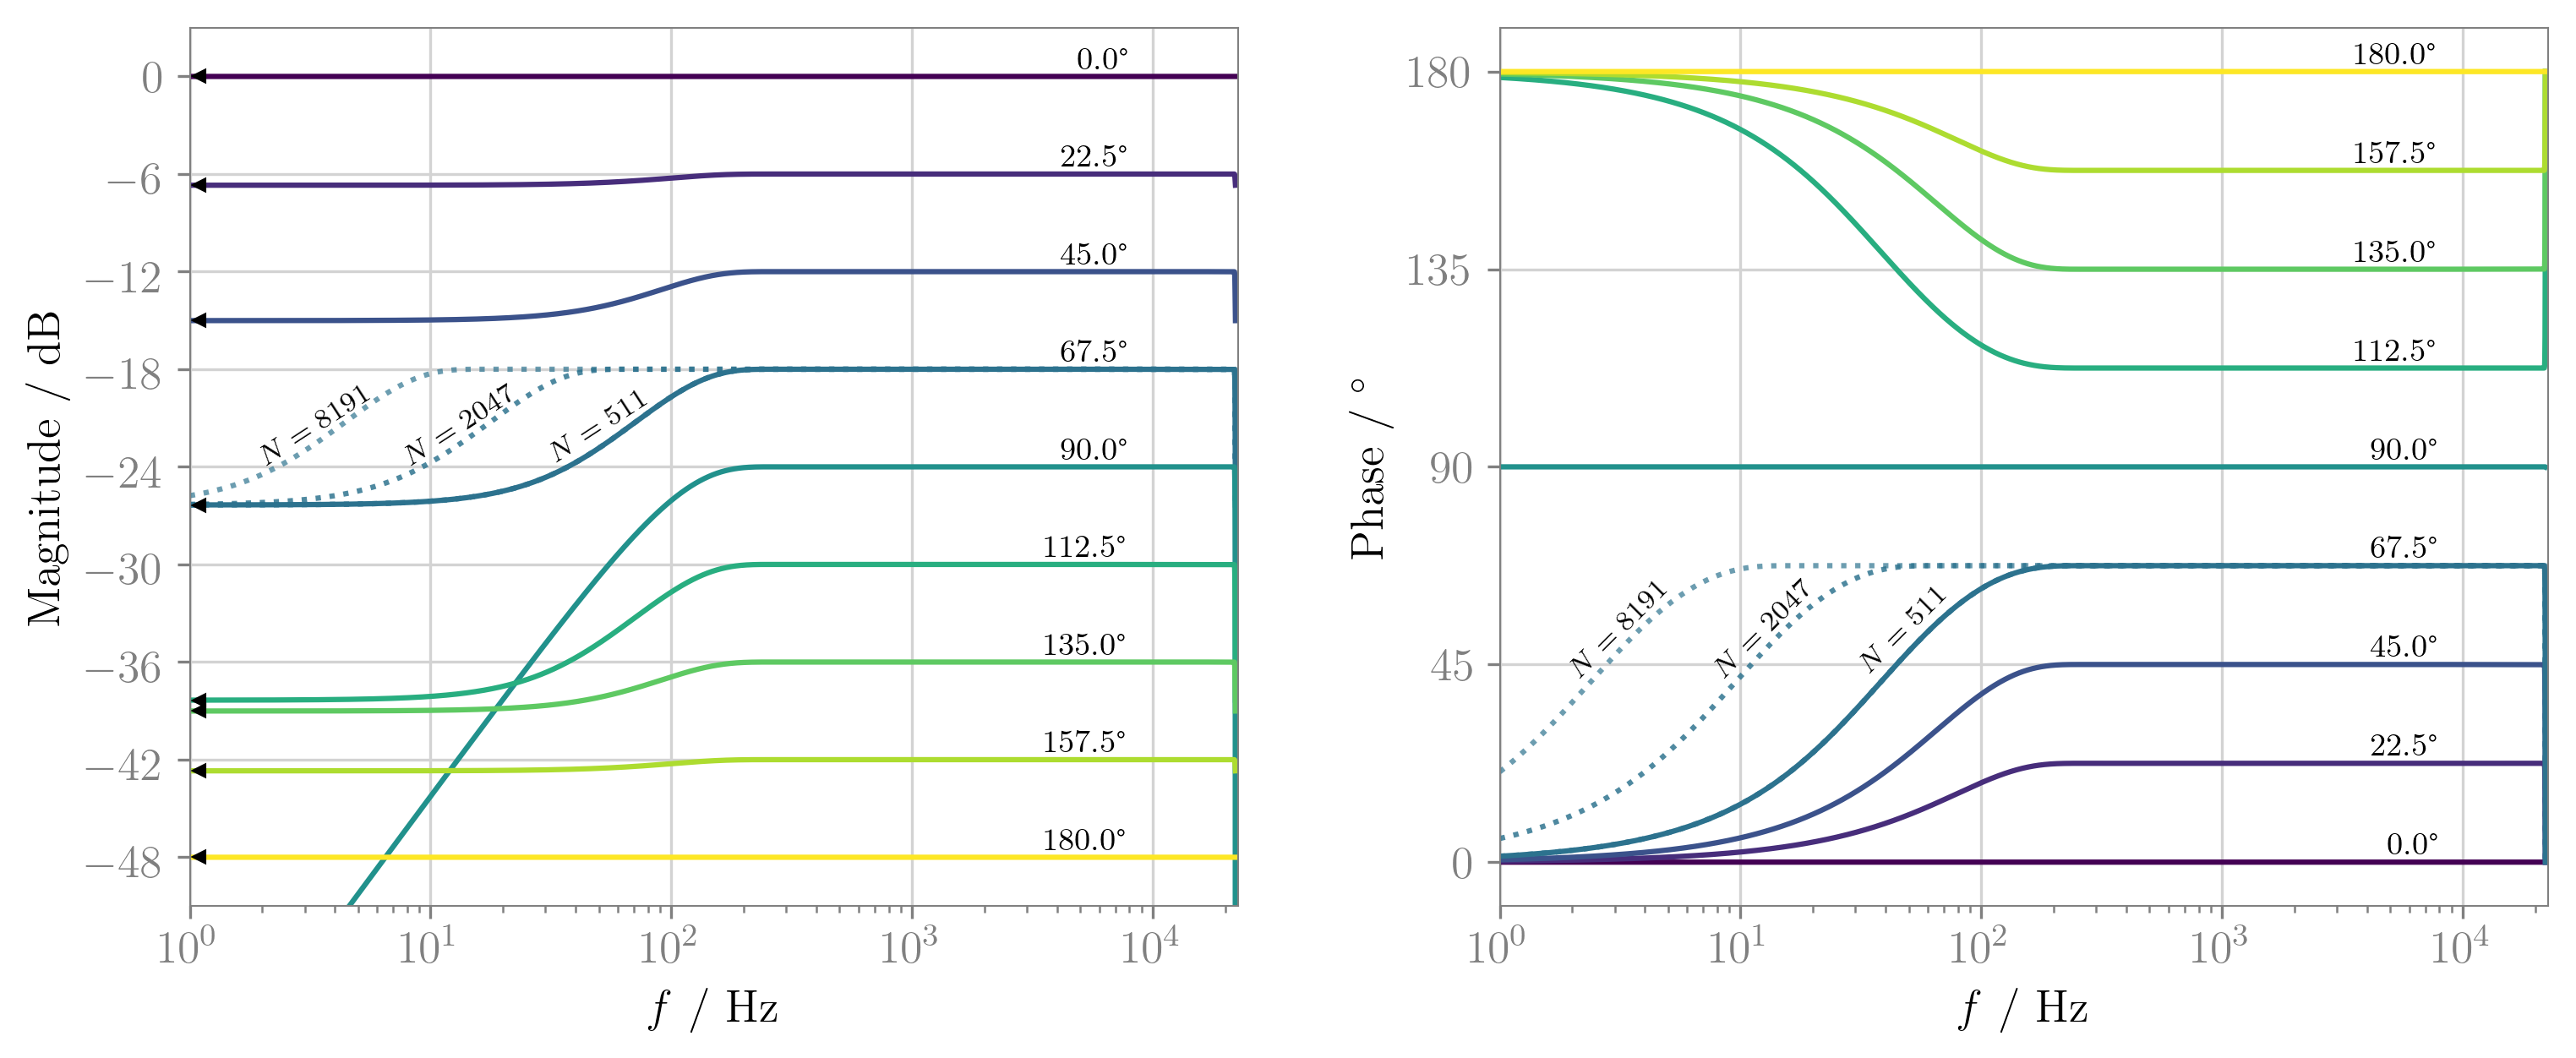
\includegraphics[width=0.85\linewidth]{graphics/spectra_filterorder510.pdf}
\caption{Frequency responses of constant phase shifters
(left: magnitude, right: phase, $\fs=44.1$~kHz).
The FIR filter coefficients are obtained by using the windowing method
(filter length of $N=511$ for all angles and $N=511, 2047, 8191$ for $\varphi=67.5\degree$).
The magnitude responses are depicted with $6$~dB offsets.
The triangles $\LHD$ indicate the DC gain $\cos\varphi$.
The phase responses are obtained by compensating the group delay
$\tau = \frac{N-1}{2}\frac{1}{\fs}$, i.e. multiplying the complex exponential
$e^{i2\pi f\tau}$ to the spectra.}
\label{fig:spectra}
\end{figure*}
%
\NewL The discrete-time impulse response of a constant phase shifter
is obtained by computing the inverse DTFT of $H(e^{i\Omega})$,
%either \eqref{eq:def-dtft} or \eqref{eq:decomp-dtft},
\begin{align}
h[n] =
\begin{cases}
\cos\varphi, & n = 0\\
0, & \text{$n \neq 0$ and even}\\
-\frac{2}{n \pi} \sin\varphi, & \text{$n$ odd}.
\end{cases}
\label{eq:discrete-ir}
\end{align}
Analogous to \eqref{eq:decomp-dtft},
it comprises of two components,
\begin{align}
h[n] &= \cos\varphi\cdot\delta[n]
- \sin\varphi \cdot \hh[n]
\label{eq:decomp-ir}
\end{align}
where
\begin{align}
\hh[n] =
\begin{cases}
0,& \text{$n$ even}\\
\tfrac{2}{n\pi},& \text{$n$ odd}.
\end{cases}
\end{align}
denotes the discrete-time impulse response of
the Hilbert transform filter~\cite[Eq.~(11.65)]{oppenheim}.
The constant phase shift of an input signal is
thus a linear combination of the input itself and its Hilbert transform,
weighted with $\cos\varphi$ and $-\sin\varphi$, respectively.
%
\NewL In Fig.~\ref{fig:discrete-ir}(left),
the impulse response $h[n]$ for $\varphi=-\tfrac{\pi}{4}$ is depicted.
It can be seen that the impulse response is
of infinite length and not causal.
The coefficients for $n\!\neq\!0$, indicated by \stem{colnonzero},
exhibit odd symmetry with respect to $n=0$ and add up to 0.
The DC and $\frac{\fs}{2}$ gain are thus solely determined by $h[0]=\cos\varphi$,
indicated by \stem{colzero}
and consistently given in \eqref{eq:def-dtft}.
%
\NewL Filtering with the impulse response $h[n]$ is not feasible in practice
due to the infinite extent of $h[n]$.
An FIR constant phase shifter can be built by applying a finite window to $h[n]$,
known as windowing method~\cite[Sec.~7.2]{oppenheim}.
Considering the decay of the coefficients for $\abs{n}\to\infty$,
it is a natural choice to truncate the impulse response
symmetrically with respect to $n=0$, which leads to
an even-order (odd-length) FIR filter.
Since $h[n]$ vanishes for even $n\neq 0$,
the FIR length $N$ has to satisfy $N\bmod 4 = 3$
(i.e. $N = 3, 7, 11, 13, \ldots$).
Using a tapering window is advantageous
as it smooths out the ripples in the frequency domain.
Due to the non-causality of the filter, a constant group delay of $\tau = \frac{N - 1}{2}\frac{1}{\fs}$
%(about the half filter length)
is introduced additionally to the desired property given by \eqref{eq:def-dtft}.
%
\NewL Exemplary frequency responses of FIR constant phase shifters
($\varphi=0\degree,\ldots,180\degree$)
are shown in Fig.~\ref{fig:spectra}.
The FIR coefficients are obtained by applying
a Blackman window to $h[n]$ in \eqref{eq:discrete-ir}.
It can be seen that the desired magnitude and phase responses
are achieved only within a limited frequency band.
For $\varphi \neq 0\degree, 180\degree$,
the magnitude responses typically
attenuate at low and high ends
($f=0$ and $f=\tfrac{\fs}{2}$, respectively)
and converge to $\cos\varphi$.
Due to the logarithmic frequency axis,
the behavior at $f=\frac{\fs}{2}$ is not clearly visible, though.
For $\varphi\neq 90\degree$,
the phase responses are inaccurate at both ends
and gradually tend to $0\degree$ or $180\degree$.
The constant phase shifter for $\varphi=90\degree$ exhibits an ideal phase response
but the most distorted magnitude response among other phase angles.
Accurate frequency responses are observed for $\varphi=0\degree, 180\degree$
where the filters are integer delays ($\tau\!=\!\frac{N-1}{2}\frac{1}{\fs}$)
with non-inverted and inverted polarity.
As indicated by dotted lines ($\varphi=67.5\degree$) in Fig.~\ref{fig:spectra},
the spectral distortions can be suppressed
by increasing the FIR filter order,
which comes at the expense of an increased group delay.

\subsection[Periodic Signals]{Periodic Signals%
\footnote{The derivation in this subsection is adopted from
\cite[Sec.~1.9 and Sec.~4.6]{hahn1996hilbert}.}}
\label{sec:periodic-signals}
%
Consider an $M$-periodic signal $\speri[n] = \speri[n + M]$
and the generating signal $s[n]$ which coincides
with $\speri[n]$ for the period $n=0,\ldots,M\!-\!1$ and vanishes elsewhere.
Then the periodic signal can be represented as a shifted sum of $s[n]$,
\begin{align}
\speri[n] = \sum_{\mu=-\infty}^{\infty} s[n] \convn \delta[n-\mu M],
\label{eq:periodic-rep}
\end{align}
where $\convn$ denotes the linear convolution with regard to $n$.
The constant phase shift of $\speri[n]$ reads
\begin{align}
\yperi[n] = \speri[n] \convn h[n]
= s[n] \convn
\underbrace{\sum_{\mu=-\infty}^{\infty} h[n-\mu M]}_{\hperi[n]},
\label{eq:periodic-conv}
\end{align}
meaning that the generating function $s[n]$ is convolved with
an infinite sum of shifted impulse responses denoted by $\hperi[n]$.
A closed form expression for $\hperi[n]$ can be obtained by
substituting \eqref{eq:decomp-ir} for $h[n]$ and exploiting
the series expansion of the cotangent function~\cite[Eq.~(4.3.91)]{abramowitz},
reading
\begin{align}
\hperi[n]=
\begin{cases}
\cos\varphi,& n=0\\
0,& \text{$n\neq 0$ and even}\\
\frac{-2\sin\varphi}{M}\cot\left(\frac{\pi n}{M}\right),& \text{$n$ odd},
\end{cases}
\label{eq:hperi-even}
\end{align}
for even $M$, and
\begin{align}
\hperi[n]=
\begin{cases}
\cos\varphi,& n=0\\
\frac{-\sin\varphi}{M} \cot\left(\frac{\pi(n + M)}{2M}\right),& \text{$n\neq 0$ and even}\\
\frac{-\sin\varphi}{M} \cot\left(\frac{\pi n}{2M}\right),& \text{$n$ odd},
\end{cases}
\label{eq:hperi-odd}
\end{align}
for odd $M$.
Exemplary impulse responses are shown
in Fig.~\ref{fig:discrete-ir}(center, right) for $\varphi=-45\degree$.
%
\NewL A periodic repetition of a signal in the time domain
is equivalent to a sampling of the spectrum in the DTFT domain~\cite[Sec.~8.4]{oppenheim}.
The discretized DTFT spectrum then constitutes
the discrete Fourier transform (DFT) spectrum~\cite[Sec.~8.5]{oppenheim},
for which periodicity of the signal and the spectrum are inherent.
The DFT coefficients for even $M$ read
\begin{align}
H[k] &= H(e^{i\frac{2\pi}{M}k})\label{eq:H-dft}\\
&= \nonumber
\begin{cases}
e^{+i\varphi},& k = 1,\ldots,\tfrac{M}{2}-1\\
e^{-i\varphi},& k = \tfrac{M}{2} + 1,\ldots, M-1\\
\cos\varphi,& k = 0, \tfrac{M}{2}
\end{cases}
\end{align}
where $H[k]$ denotes the DFT of $\hperi[n]$.
Note that \eqref{eq:hperi-even}, \eqref{eq:hperi-odd}, and \eqref{eq:H-dft}
are analytic representations of the constant phase shifter
with no approximations involved.
An ideal constant phase shift is therefore feasible
as far as periodic discrete-time signals are concerned.
%
\NewL In practice, a constant phase shift of a periodic signal
can be computed efficiently in the DFT domain,
\begin{align}
y[n] = \frac{1}{M} \sum_{k=0}^{M-1} S[k] \: H[k] \: e^{i\frac{2\pi}{M}kn},
\label{eq:dft-conv}
\end{align}
for $n=0,\ldots,M-1$, where $S[k]$ denotes the DFT of $s[n]$.
This constitutes a circular convolution of $s[n]$ and $\hperi[n]$,
and $y[n]$ exhibits a temporal aliasing which constitutes the desired result,
as shown in \eqref{eq:periodic-conv}.
Finally, the periodic signal $\yperi[n]$ is constructed
with the generating signal $y[n]$, in the same way as \eqref{eq:periodic-rep}.
